%%%%%%%%%%%%%%%%%%%%%%%%%%%%%%%%%%%%%%%%
%% Formato para revista ASOiMAT basado en la clase
%% aleph-revista, versión 1.0 (13/06/2021)
%%%%%%%%%%%%%%%%%%%%%%%%%%%%%%%%%%%%%%%%
\documentclass{aleph-revista}

%%%%%%%%%%%%%%%%%%%%%%%%%%%%%%%%%%%%%%%%
%% Declaración de paquetes adicionales
%%%%%%%%%%%%%%%%%%%%%%%%%%%%%%%%%%%%%%%%
%% Aquí incluya los paquetes necesarios para su documento. 
%% No incluya paquetes que no sean necesarios. 
%% Estos son ejemplos de paquetes que le pueden ser de utilidad.
%% Si no los va a utilizar, eliminarlos.
\usepackage{tikz}           % Para generar gráficos 
\usepackage{aleph-comandos} % Comandos para facilitar escritura matemática
\usepackage{multicol}       % Para utilizar multicolumnas
\addbibresource{Bibliografia.bib}         % Archivo de bibliografía

%%%%%%%%%%%%%%%%%%%%%%%%%%%%%%%%%%%%%%%%
%% Declaración de comandos adicionales
%%%%%%%%%%%%%%%%%%%%%%%%%%%%%%%%%%%%%%%%
%% Aquí incluya los definiciones de comandos necesarios para 
%% su documento.
%%%%%%%%%%%%%%%%%%%%%%%%%%%%%%%%%%%%%%%%
%% Datos del la publicación
%%%%%%%%%%%%%%%%%%%%%%%%%%%%%%%%%%%%%%%%
\volumen{1}
\numero{1}
\fechapubli{2021}
\periodouno{Marzo}
\periododos{Junio}
%%%%%%%%%%%%%%%%%%%%%%%%%%%%%%%%%%%%%%%%
%% Datos del artículo
%%%%%%%%%%%%%%%%%%%%%%%%%%%%%%%%%%%%%%%%
\titulo{ANÁLISIS DE VIBRACIONES LIBRES EN ROBOT KR 1000 TITAN}

\tituloingles{FREE VIBRATIONS ANALYSIS IN ROBOT KR 1000 TITAN}

\autor{%
    Bustillo, Carlos\textsuperscript{1 \faEnvelopeO}; 
    Linares, Ramiro\textsuperscript{1\faEnvelopeO}; 
    Pérez, Rodrigo\textsuperscript{1\faEnvelopeO}
}

\institucion{
\textsuperscript{1}%
    Facultad de Ingeniería, Universidad Nacional de Cuyo, Mendoza, Argentina
}

\correo{cabustillo13@hotmail.com;   rodrigoperez2110@gmail.com; ramylinares@gmail.com}

\fecha{27 de junio de 2021}

\resumen{
   El KR 1000 TITAN es un robot industrial de 6 GDL diseñado para trabajar con cargas pesadas a elevada rapidez y precisión, hasta una distancia de 6,5 m. Se lo utiliza para manipular bloques de motor, piedras, piezas de vidrio, vigas de acero, piezas navales y aeronáuticas, bloques de mármol o prefabricados de hormigón, entre otros muchos. Nuestro análisis onsiste en realizar un estudio vibratorio, para poder asegurar que las oscilaciones producidas no sean demasiado grandes como para interferir en la operación que lleve a cabo el robot en dicha posición. Al agarrar un objeto, se le suma su masa a la del sistema, y se determinará cómo esto influye en su vibración libre.
 
}
\palabrasc{Robot KUKA, Vibraciones Libres, Modos de vibración.}

\abstract{
    The KR 1000 TITAN is a 6 DOF industrial robot designed to work with heavy loads at high speed and precision, up to a distance of 6.5 m. It is used to manipulate engine blocks, stones, glass pieces, steel beams, naval and aeronautical pieces, marble blocks or precast concrete, among many others. Our analysis consists in carrying out a vibratory study, in order to ensure that the oscillations produced are not too large to interfere with the operation carried out by the robot in that position. When grasping an object, its mass is added to that of the system, and it will be determined how this influences its free vibration.
}
\keywords{KUKA robot, Free Vibrations, Vibration modes.}

\begin{document}
%%%%%%%%%%%%%%%%%%%%%%%%%%%%%%%%%%%%%%%%
%% Encabezado
%%%%%%%%%%%%%%%%%%%%%%%%%%%%%%%%%%%%%%%%
\membrete
%%%%%%%%%%%%%%%%%%%%%%%%%%%%%%%%%%%%%%%%
\section{Introducción}
%%%%%%%%%%%%%%%%%%%%%%%%%%%%%%%%%%%%%%%%
La revista \asoimat{}, es una revista electrónica de publicación trimestral que se dedica a la publicación de artículos periodísticos y científicos de las matemáticas puras, aplicadas y ciencias afines a estas. El proceso de publicación de un artículo requiere la revisión de pares previo a su publicación.

Por otra parte, todos los artículos publicados en la revista \asoimat son de libre acceso sin restricciones económicas o de contenido de manera electrónica o física. Para más información se recomienda leer la guía para autores disponible en el sitio web de la revista: \url{https://revistaasoimat.epn.edu.ec/index.php/ASOiMAT/information/authors}.


%%%%%%%%%%%%%%%%%%%%%%%%%%%%%%%%%%%%%%%%
\section{Derechos de autor}
%%%%%%%%%%%%%%%%%%%%%%%%%%%%%%%%%%%%%%%%

Los artículos publicados en la revista \asoimat se encuentran sujetos a la licencia: Atribución - NoComercial - CompartirIgual 4.0 Internacional (CC BY-NC-SA 4.0). Para más información, puede visitar: \url{https://creativecommons.org/licenses/by-nc-sa/4.0/}. 

%%%%%%%%%%%%%%%%%%%%%%%%%%%%%%%%%%%%%%%%
\section{Requerimientos técnicos}
%%%%%%%%%%%%%%%%%%%%%%%%%%%%%%%%%%%%%%%%

A continuación se encuentra una lista con los requerimientos técnicos que debe tener el documento.

\begin{enumerate}
\item 
    Los artículos deben estar escritos en \LaTeX{} con la presente plantilla que se encuentra en libre distribución para su uso.
\item 
    Al momento de presentar el artículo no debe realizar ninguna manipulación de estilo (alinear textos, tamaño de letra, etc.). El único formato admitido para énfasis de texto es la \textit{itálica}. Las palabras en otro idioma deben ir siempre en \textit{itálica}. (Se recomienda el uso del comando \verb|\emph| para este propósito.)
\item 
    Las imágenes deben estar en formato \texttt{JPG}, \texttt{PNG}, \texttt{PDF} o \texttt{EPS}, con una resolución apropiada a la presentación.
\item 
    Las imágenes deben archivos \texttt{.jpg}, \texttt{.png}, \texttt{.pdf} o\texttt{.eps}, con una resolución apropiada a la presentación.
\item 
    Escriba el código fuente de manera clara y ordenada, usando comentarios si requiere sugerir un formato o diseño específico para la publicación de su trabajo. 
\item 
    En el caso de generar nuevos comandos o ambientes, estos deben colocarse en el preámbulo del documento en la sección destinada para este fin.
\end{enumerate}

%%%%%%%%%%%%%%%%%%%%%%%%%%%%%%%%%%%%%%%%
\section{Partes del documento}
%%%%%%%%%%%%%%%%%%%%%%%%%%%%%%%%%%%%%%%%

El artículo a presentarse debe contener las siguientes partes:

\subsection{Título}

El título del artículo debe ser corto y conciso.

\subsection{Nombres de los autores y filiación}

El nombre o los nombres de los autores deben ser incluidos en el apartado destinado para este caso, junto con su filiación. Se debe agregar solo uno de los autores como contacto de correspondencia y este debe estar señalado con el ícono correspondiente.

\subsection{Listas}

Las listas se construyen de manera sencilla llamando al ambiente predeterminado para estas, no se deben modificar los parámetros de la misma ni el estilo. Ejemplos de listas y enumeraciones se encuentran a continuación:

\begin{multicols}{2}
\paragraph{Listas}
\begin{itemize} 
    \item Punto 1
    \item Punto 2
    \item Punto 3
\end{itemize}

\paragraph{Enumeraciones}
\begin{enumerate} 
    \item Punto 1
    \item Punto 2
    \item Punto 3
\end{enumerate}

\end{multicols}

En el caso de que las listas o enumeraciones de numerosos ítems de longitud, se deben usar varias columnas para un mejor ajuste. Por ejemplo:

\subsubsection{Listas} 

\begin{multicols}{3}
\begin{itemize} 
    \item Punto 1
    \item Punto 2
    \item Punto 3
    \item Punto 4
    \item Punto 5
    \item Punto 6
    \item Punto 7
    \item Punto 8
    \item Punto 9
\end{itemize}
\end{multicols}

\subsubsection{Enumeraciones}
\begin{multicols}{3}
\begin{enumerate} 
    \item Punto 1
    \item Punto 2
    \item Punto 3
    \item Punto 4
    \item Punto 5
    \item Punto 6
    \item Punto 7
    \item Punto 8
    \item Punto 9
\end{enumerate}
\end{multicols}

Para el desarrollo de listas y enumeraciones anidadas, se recomienda un máximo de 3 niveles de anidación. Ejemplos de dichas anidaciones se encuentran a continuación:

% \begin{multicols}{2}
\paragraph{Listas}
\begin{enumerate}
    \item Punto 1
    \item Punto 2 \begin{enumerate}
        \item Punto 2.1
        \item Punto 2.2 \begin{enumerate}
            \item Punto 2.2.1
        \end{enumerate}
    \end{enumerate}
\end{enumerate}

\paragraph{Enumeraciones}
\begin{itemize}
    \item Punto 1
    \item Punto 2 \begin{itemize}
        \item Punto 2.1
        \item Punto 2.2 \begin{itemize}
            \item Punto 2.2.1
        \end{itemize}
    \end{itemize}
\end{itemize}

% \end{multicols}

%%%%%%%%%%%%%%%%%%%%%%%%%%%%%%%%%%%%%%%%
\section{Figuras}
%%%%%%%%%%%%%%%%%%%%%%%%%%%%%%%%%%%%%%%%

Las figuras aceptadas incluyen tanto gráficos creados en TikZ, PSTricks como imágenes de mapas de bits.

\subsection{TikZ}

Por defecto, se recomienda emplear el lenguaje TikZ para el desarrollo de figuras. Los paquetes necesarios para este fin deben ser incluidos en el documento principal.

\begin{figure}[H]
    \centering
    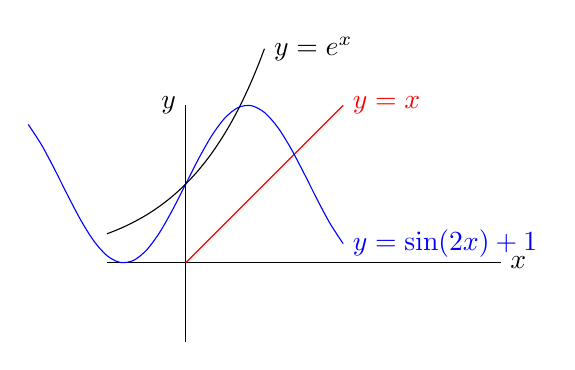
\begin{tikzpicture}
    \draw (-1,0) -- (4,0) node[right] {$x$};
    \draw (0,-1) -- (0, 2) node[left] {$y$};
    \draw[smooth, domain = 0:2, color=red] plot (\x,\x)node[right] {$y = x$
    };
    \draw[smooth, domain = -2:2, color=blue] plot (\x,{sin(2*\x r)+1})
    node[right] {$y = \sin(2x)+1$};
    \draw[smooth, domain = -1:1, color=black] plot (\x,{exp(\x)}) node[right
    ] {$y = e^x$};
    \end{tikzpicture}
    \caption{Gráfico}
    \label{fig:grafico2}
\end{figure}

\subsection{PSTrciks}

Aunque se recomienda TikZ, el autor puede optar por usar PSTricks. En este caso, debe asegurarse de que las imágenes adjuntadas se encuentren en formato \texttt{EPS}.

\subsection{Imágenes}

Las imágenes a ser incluidas pueden ser dibujos, mapas o fotografías con una resolución deseada de 300~dpi sin fondo; además, deben ser almacenadas en una carpeta separada con un nombre corto que permita su identificación.

El autor del artículo es responsable de verificar los derechos de autor de las imágenes que se envían como parte del artículo.

\begin{figure}[H]
    \centering
    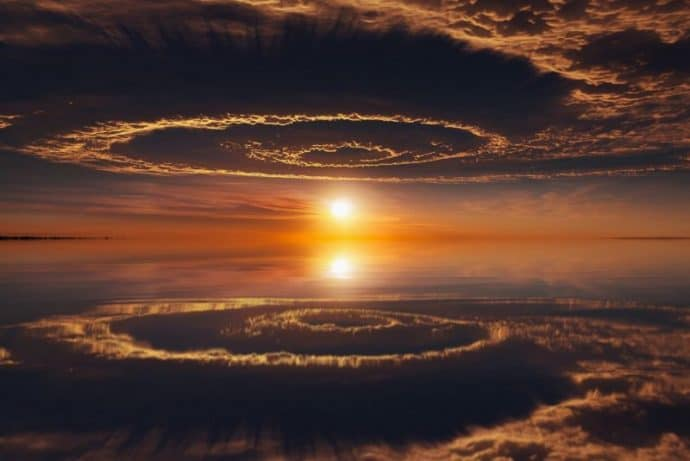
\includegraphics[width=0.60\textwidth]{Imagenes/Imagen1.jpeg}
    \caption{Leyenda de la figura.}
    \label{fig:etiqueta de la figura}
\end{figure}

Se recomienda que la imagen no ocupe más del 50\% de la página salvo que así lo requiera por sus dimensiones. Un tamaño recomendado es un ancho del 75\% de la línea de texto con una altura proporcional a la primera.

Todas las imágenes deben incluir una leyenda y en el caso de hacer referencia a las mismas, se deben usar referencias cruzadas para este fin, es decir, los comandos: \verb@\label@ y \verb@\ref@.




%%%%%%%%%%%%%%%%%%%%%%%%%%%%%%%%%%%%%%%%
\section{Desarrollo de las ecuaciones de Lagrange}
%%%%%%%%%%%%%%%%%%%%%%%%%%%%%%%%%%%%%%%%

\subsection{Para \theta_1}

\begin{flalign*}
    &\frac{\partial(U)}{\partial(\theta_1)} = \theta_1[k_1 + k_2 - m_1g\frac{R}{2} - (m_3 + m_4)g(R-dcm_3_4) + \theta_2(-k_2)]&
\end{flalign*}

\begin{flalign*}
    &\frac{\partial(D)}{\partial(\dot{\theta_1})} = \dot{\theta_1}(c_1 + c_2) + \dot{\theta_2}(-c_2)&
\end{flalign*}

\begin{flalign*}
    &\frac{d(T)}{dt(\dot{\theta_1})} = J_1_Y\ddot{\theta_1} +  \ddot{\theta_1}(m_1)\frac{R^2}{4} + \frac{1}{2}m_2[ 2R^2\ddot{\theta_1} -V\ddot{\theta_2}R(cos\theta_2sen\theta_1 - cos\theta_1sen\theta_2)] + &\\ &\frac{1}{2}(m_3+m_4)[2R^2\ddot{\theta_4} - [2dcm_3_4\ddot{\theta_3}Rsen\theta_1sen\theta_3 + 2\ddot{\theta_2}VRcos\theta_2sen\theta_1 - 2dcm_3_4\ddot{\theta_3}Rcos\theta_1cos\theta_3]]&
\end{flalign*}

\begin{flalign*}
    &\frac{\partial(T)}{\partial(\theta_1)} = -\frac{1}{2}m_2VR\dot{\theta_1}\dot{\theta_2}(sen\theta_2sen\theta_1 - cos\theta_2cos\theta_1) -\frac{1}{2}(m_3+m_4)[ 2\dot{\theta_1}dcm_3_4\dot{\theta_3}Rcos\theta_1sen\theta_3 +&\\
    &(2\dot{\theta_1}\dot{\theta_2}VRsen\theta_2 - 2\dot{\theta_1} dcm_3_4\dot{\theta_3}Rcos\theta_3)sen\theta_1 + 2\dot{\theta_1}\dot{\theta_2}VRcos\theta_2cos\theta_1 ]&
\end{flalign*}




\subsection{Ambientes matemáticos}
Están incluidos los siguientes ambientes:
\begin{itemize}
    \item Definición (\texttt{defi});
    \item Teorema (\texttt{teo});
    \item Proposición (\texttt{prop});
    \item Lema (\texttt{lema});
    \item Axioma (\texttt{axioma}).
\end{itemize}
Algunos ejemplos se pueden encontrar a continuación:

\begin{defi}[Razón de cambio promedio]
    Sea $\func{f}{I}{\R}$ una función, $a\in I$ y $h\in\R$ tal que $a+h\in I$, se define \emph{la razón de cambio promedio de la función $f$ entre $a$ y $a+h$} por
    \[
        \frac{f(a+h)-f(a)}{h}.
    \]
    Este número también es conocido como \emph{variación media} de $f$ en el intervalo que une $a$ y $a + h$.
\end{defi}

\begin{prop}
    Sean $\func{f}{I}{\R}$ una función y $a\in I$. Se tiene que $f$ es derivable en $a$ si y solo si existe
    \[
        \lim_{x\to a}\frac{f(x)-f(a)}{x-a}.
    \]
\end{prop}

\begin{lem}
    Sean $a,p\in\N$, con $p$ un primo. Si $a^2$ es un múltiplo de $p$, entonces $a$ también es un múltiplo de $p$.
\end{lem}

\begin{axioma}[Axiomas de Peano]
    El conjunto de los números naturales, está caracterizado por las siguientes propiedades:
    \begin{enumerate}
    \item
        El conjunto $\N$ es no vacío, posee al elemento 1.
    \item
        Todo número natural posee un sucesor.
    \item
        Dados dos números $n,m\in\N$ con el mismo sucesor, entonces $n=m$.
    \item
        El número 1 no es sucesor de ningún otro elemento de $\N$.
    \item
        Los números naturales son un conjunto inductivo.
    \end{enumerate}
\end{axioma}

Las demostraciones deben ser escritas en el ambiente \texttt{proof} con la siguiente sintaxis:

\begin{lstlisting}[language=TeX]
\begin{proof}
% Aquí escriba la demostración
%
% Use el comando \qedhere para un mejor ajuste
\end{proof}
\end{lstlisting}

Para una mejor redacción matemática se sugiere leer: \url{http://www.texnia.com/archive/ortomatem.pdf}. Para una escritura más sencilla de fórmulas y desarrollos matemáticos se puede usar el paquete \texttt{aleph-comandos} que se encuentra en: \url{https://git.alephsub0.org/}. 

%%%%%%%%%%%%%%%%%%%%%%%%%%%%%%%%%%%%%%%%
\section{Tablas}
%%%%%%%%%%%%%%%%%%%%%%%%%%%%%%%%%%%%%%%%

Para la composición de tablas, la letra siempre debe ser de tamaño menor a la del resto del texto y se recomienda optar por el siguiente formato:

\begin{table}[H]
    \centering\small
    \begin{tabular}{ccc}
    \toprule
        \textbf{Fórmula} & \textbf{Prueba 1} & \textbf{Prueba 2} \\ 
    \midrule
        Compuesto 1 & $38.4$  &  $6.32$\\ 
        Compuesto 2 & $16.6$ & $12.5$ \\ 
    \bottomrule
    \end{tabular}
    \label{tab:01}
    \caption{Resultados de la experimentación de distintas substancias.}
\end{table}

Las tablas, al igual que las figuras, siempre deben poseer una leyenda y en el caso de ser referenciadas dentro del documento, deben hacer uso de referencias cruzas, es decir, los comandos: \verb@\label@ y \verb@\ref@.


Este hace uso del paquete \texttt{booktabs} que mejora la presentación de las mismas y usa los comandos \verb@\toprule@, \verb@\midrule@ y \verb@\bottomrule@.

%%%%%%%%%%%%%%%%%%%%%%%%%%%%%%%%%%%%%%%%
\section{Enlaces}
%%%%%%%%%%%%%%%%%%%%%%%%%%%%%%%%%%%%%%%%

Para la inclusión de direcciones URL, se recomienda el uso del comando \verb@\url@, únicamente en caso de que el enlace sea extenso o complejo, se puede reemplazar por el comando \verb@\href@.

%%%%%%%%%%%%%%%%%%%%%%%%%%%%%%%%%%%%%%%%
\section{Código}
%%%%%%%%%%%%%%%%%%%%%%%%%%%%%%%%%%%%%%%%

Para la inclusión de código se debe usar el paquete \texttt{listing} y para pseudocódigo, \texttt{algorithm2e}; estos paquetes ya se encuentra cargado en la clase y un ejemplo de pseudocódigo y código se encuentra a continuación. Se debe incluir leyendas de cada código y pseudocódigo.

\subsection{Pseudocódigo} 

Ejemplo de pseudocódigo.

\begin{algorithm}[H]
\KwData{Dos números reales $a$ y $b$}
\KwResult{El máximo entre $a$ y $b$}
\SetKwFunction{maxi}{Máximo}
\Fn{\maxi{$a,b$}}{
    \eIf{ $a < b$}
        {\Return{$b$}}
        {\Return{$a$}}
    }
\caption{Ejemplo de Pseudocódigo.}
\end{algorithm}

\subsection{Código}

Ejemplo de código.

\begin{lstlisting}[language=Python,caption={Ejemplo de código.},captionpos=b]]
def OrdenBurbuja(a):
    for i in range(len(a)-2):
        for j in range(len(a)-i-1):
            if a[j] > a[j+1]:
                a[j],a[j+1] = a[j+1],a[j]
    return a
\end{lstlisting}

%%%%%%%%%%%%%%%%%%%%%%%%%%%%%%%%%%%%%%%%
\section{Bibliografía y citas}
%%%%%%%%%%%%%%%%%%%%%%%%%%%%%%%%%%%%%%%%

La bibliografía debe incluirse mediante un archivo \texttt{.bib} con el mismo nombre que el archivo principal y utilizando el paquete \texttt{biblatex} (ya incluido en la clase). Únicamente deben incluirse referencias citadas en el artículo.

El estilo bibliográfico a usar es APA séptima edición, algunos ejemplos e información se pueden encontrar en: \url{https://apastyle.apa.org/style-grammar-guidelines/references/examples}. Y una versión traducida en: \url{https://normasapa.pro/}.

Para las citas puede utilizar los siguientes comandos según sea adecuado:
\begin{itemize}
\item 
    Cita completa entre paréntesis \verb"\parencite{ }": \parencite{Bib06}
\item
    Cita completa sin paréntesis \verb"\textcite{ }": \textcite{Bib06}
\item 
    Cita completa entre paréntesis \verb"\cite{ }": \cite{Bib06}
\item
    Cita de autor \verb"\citeauthor{ }": \citeauthor{Bib06}
\item
    Cita de año \verb"\citeyear{ }": \citeyear{Bib06}
\item 
    Cita con opciones extras \verb"\parencite[ ][ ]{ }": \parencite[ver][pág. 66]{Bib06}
\end{itemize}
Información adicional sobre el paquete \texttt{biblatex} puede encontrarse en: \url{http://tug.ctan.org/info/biblatex-cheatsheet/biblatex-cheatsheet.pdf}

Finalmente, se presentan ejemplos de referencias que se pueden utilizar:
\begin{itemize}
    \item Artículos de revista: \cite{Bib01}
    \item Libros: \cite{Bib02}
    \item Libros: \cite{Bib06}
    \item Tesis: \cite{Bib03}
    \item Sitios web: \cite{Bib04}
    \item Videos: \cite{Bib05}
\end{itemize}

%%%%%%%%%%%%%%%%%%%%%%%%%%%%%%%%%%%%%%%%
\section{Comentarios}
%%%%%%%%%%%%%%%%%%%%%%%%%%%%%%%%%%%%%%%%

El presente formato se base en la clase \texttt{aleph-revista}, generada dentro del proyecto Alephsub0 (\url{https://alephsub0.org/}). Tanto el formato como la clase se encuentran en desarrollo, cualquier reporte de problema o sugerencia de mejora se lo puede realizar al siguiente correo: 
\email{daniel.lara@alephsub0.org}.


%%%%%%%%%%%%%%%%%%%%%%%%%%%%%%%%%%%%%%%%
%% Referencias
%%%%%%%%%%%%%%%%%%%%%%%%%%%%%%%%%%%%%%%%
\printbibliography



\end{document}